
\section{Analisi del prodotto esistente}
\hl{sezione nuovissima}

Al momento dell'arrivo in azienda è già presente una versione alpha del software. \\
Sono attualmente supportate le aziende con i codici \gls{ATECO} in ambito edilizio, permettendo di gestire le informazioni relative a:
\begin{itemize}
	\item Sedi;
	\item Cantieri;
	\item Dipendenti;
	\item Organigramma aziendale;
	\item Abitabilità;
	\item Certificato di prevenzione degli incendi;
	\item \gls{DVR} e documentazione collaterale ad esso.
\end{itemize}
Il software espone una collezione di oltre 400 domande. Sulla base delle risposte a queste domande ed alle informazioni relative alle entità sopra indicate, vengono verificate alcuni vincoli mediante delle regole del sistema esperto.


\hl{[TODO ]}

\subsection{Architettura del software}
\subsubsection{Architettura ad alto livello}
\hl{sezione nuovissima}
Il software è gestito mediante tecnologia , un modello di distribuzione del software applicativo dove il fornitore del software si occupa della sua implementazione e manutenzione. Il servizio viene erogato al cliente mediante una applicazione web fruibile via internet. \\ 
L'applicazione web risiede fisicamente su una macchina virtuale della piattaforma cloud \gls{AWS}, al fine di evitare oneri e spese di gestione di una infrastruttura informatica dedicata.\\

Come è possibile osservare da \autoref{fig:Architettura}, ogni istanza di macchina virtuale contiene una infrastruttura dedicata. Questo perché è prevista la possibilità di vendere il pacchetto a più utenti che possono fungere da distributori.\\
Ogni istanza è composta da tre componenti principali:
\begin{itemize}
	\item Rule Engine;
	\item Database;
	\item Storage.
\end{itemize}
Il routing delle richieste viene effettuato con un \gls{reverse proxy}, nello specifico \textit{NGINX}. \\
In particolare Ruby on Rails permette nativamente di creare e versionare i database a seconda dell'ambiente nel quale si opera (\textit{development, test, staging e production}). Questo è tornato molto utile per lo sviluppo poiché è stato possibile fare test accurati senza intaccare i dati in produzione o utilizzare la console in sandbox di Rails che presenta criticità nella sincronizzazione dei dati.
\begin{figure}[H]
	\begin{center}
		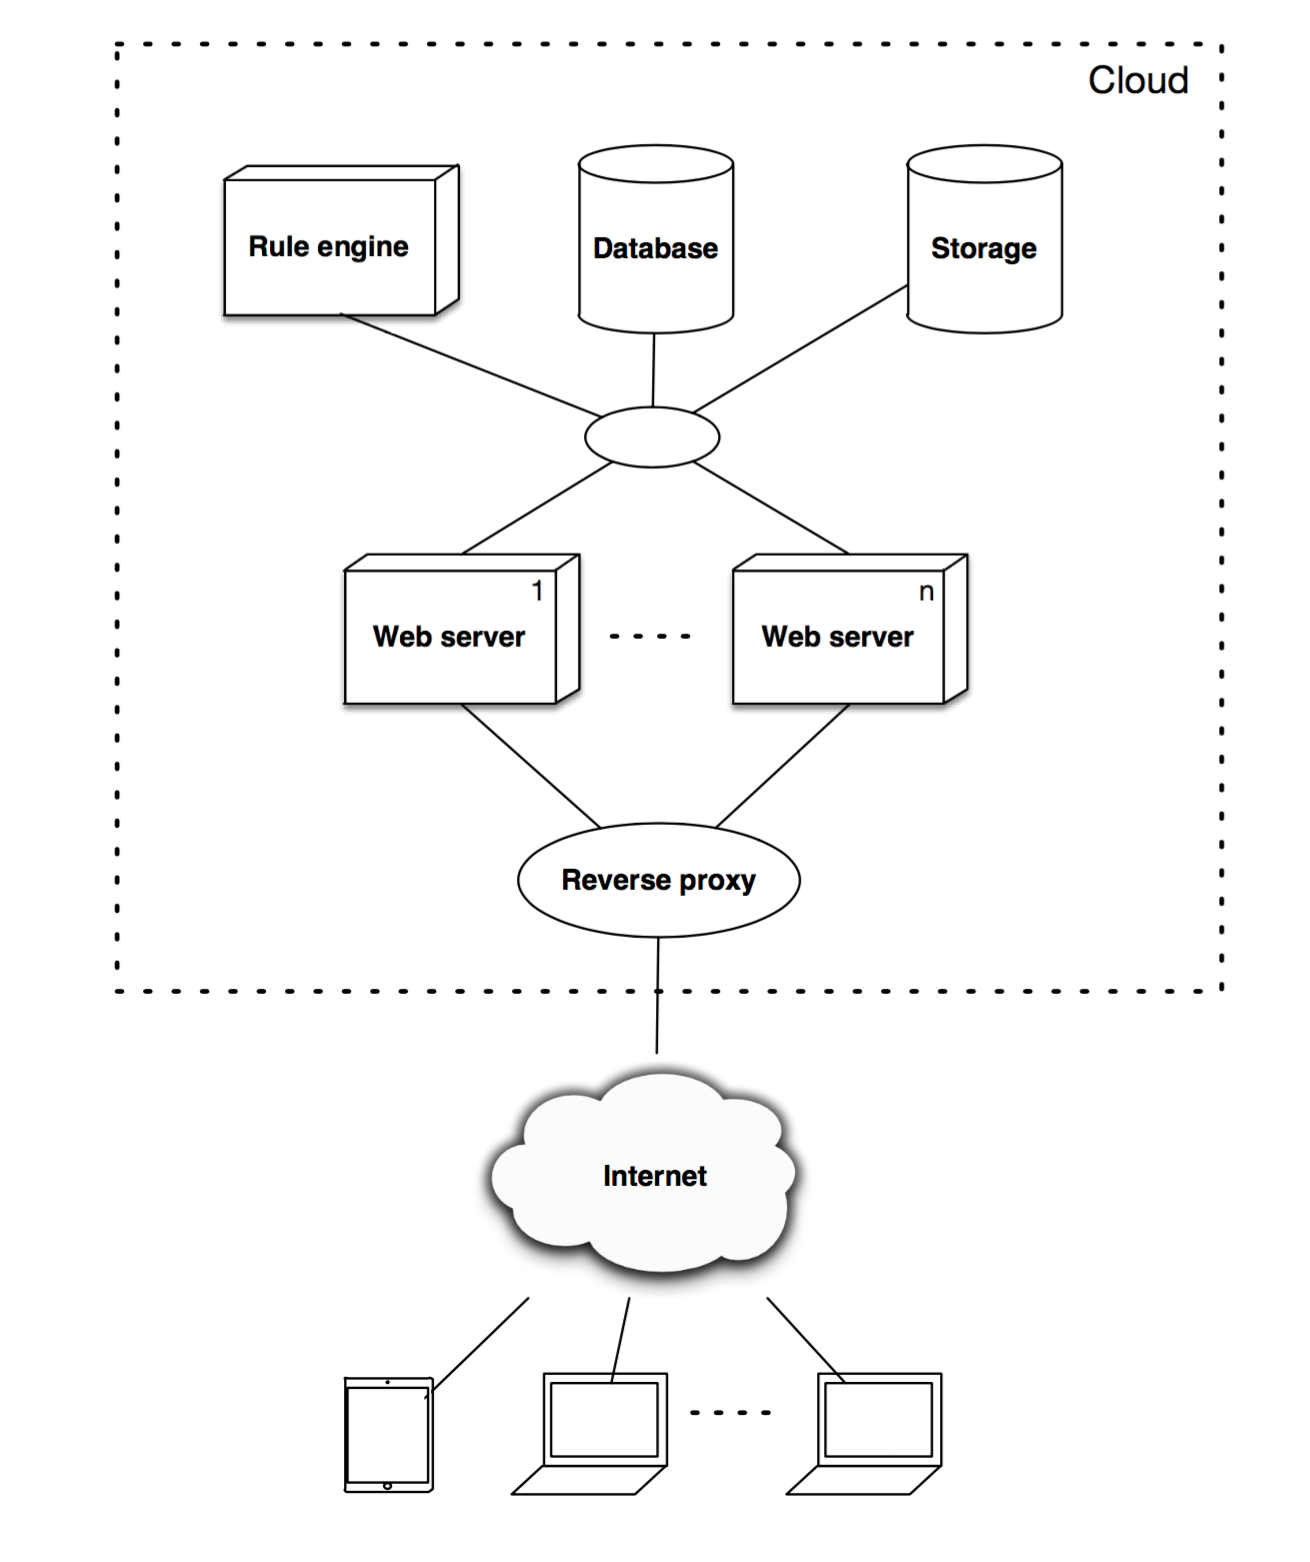
\includegraphics[width=12cm]{Pics/architettura.png}
		\caption{Architettura del sistema}
		\label{fig:Architettura}
	\end{center}
\end{figure}
\hl{SPIEGARE MEGLIO}
\subsubsection{Architettura a basso livello}

Per la realizzazione di questa applicazione web è stato utilizzato il pattern \gls{MVC}. Per il raggiungimento delle viste e l'accesso alle informazioni necessarie al corretto funzionamento dell'applicazione è stata implementata una interfaccia \gls{REST}. \\
\hl{Mettere diagramma delle classi approssimativo}\\
Il sistema ha come radice l'entità \texttt{Company} alla quale sono riferite, direttamente o indirettamente, tutte le risorse.\\ Sono poi presenti numerosi modelli relativi alle risorse che partecipano alla procedura di asseverazione. Le entità principali sono:
\begin{itemize} 
	%\setlength{\itemsep}{0pt}
	%\setlength{\parskip}{0pt}
	%\setlength{\parsep}{0pt} 
	
	\item \texttt{Alert} per rappresentare gli allarmi;
	\item \texttt{Answer} per rappresentare le risposte alle domande;
	\item \texttt{Company} per rappresentare una azienda;
	\item \texttt{ConstructionSite} per rappresentare un cantiere;
	\item \texttt{Dpi} per rappresentare un dispositivo di protezione individuale;
	\item \texttt{Duty} per rappresentare una mansione;
	\item \texttt{FireExtinguisher}  per rappresentare un estintore;
	\item \texttt{FirstAidBox} per rappresentare una cassetta di primo soccorso;
	\item \texttt{Individual} per rappresentare una persona;
	\item \texttt{Location} per rappresentare un edificio aziendale, ovvero una sede operativa, una sede amministrativa, una sede legale oppure un magazzino;
	\item \texttt{Machine, LiftingEquipment, ElectricTool}  per rappresentare un mezzi oppure uno strumento presente nel parco macchine;
	\item \texttt{Medicalvisit} per rappresentare una visita medica;
	\item \texttt{Procedure} per rappresentare una procedura aziendale, sia essa di prassi o di sistema;
	\item \texttt{Question} per rappresentare una domanda;
	\item \texttt{Training} per rappresentare un corso.
\end{itemize}	
\hl{[TODO finire di spiegare l'architettura ]}\\
Una criticità incontrata è stata quella dell'associazione di una risposta o di un \textit{allarme} alla relativa risorsa. Per fare ciò si è utilizzato l'approccio di Rails per il supporto del polimorfismo, come si può vedere da  \autoref{fig:DiagrammaClassiAssociazioniPolimorfe}. Nello specifico viene indicato il tipo e l'id della risorsa e l'accesso avviene tramite valutazione della classe e ricerca del relativo \textit{id}. \\
Si può pensare, ad esempio, all'allarme scatenato alla scadenza di un estintore. 
La Risposta (\textit{Answer}) avrà i due campi \texttt{answerable\_type} ed \texttt{answerable\_id} impostati a \textit{"FireExtinguisher"} ed al suo \textit{id} rispettivamente.  L'allarme avrà un riferimento a questa domanda, in questo modo è possibile conoscere il punto esatto dove dirottare l'utente al click sull'allarme per raggiungere il punto di non conformità. Questo aspetto è stato considerato di fondamentale importanza poiché la mole delle informazioni nel software è molto grande, è quindi necessario fornire il maggior numero di strumenti possibili all'utente per facilitare la navigazione e l'orientamento nel sistema.
\begin{figure}[H]
	\begin{center}
		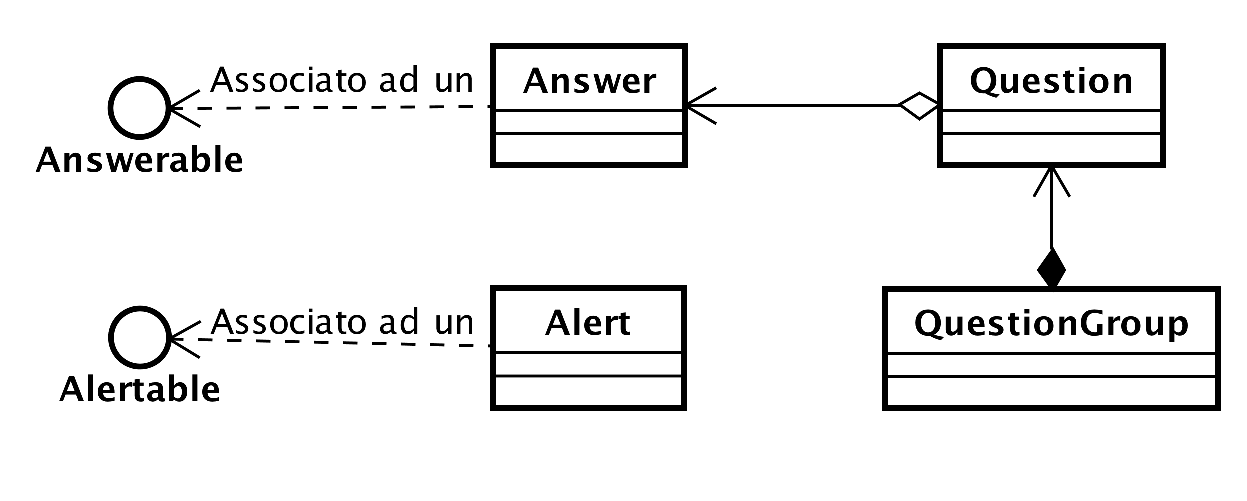
\includegraphics[width=14cm]{Pics/diagramma_classi_associazioni_polimorfe.png}
		\caption{Diagramma delle classi delle associazioni polimorfe di Risposte ed Allarmi.}
		\label{fig:DiagrammaClassiAssociazioniPolimorfe}
	\end{center}
\end{figure}



\subsubsection{Flusso dei dati ed interazione}

\begin{figure}[H]
	\begin{center}
		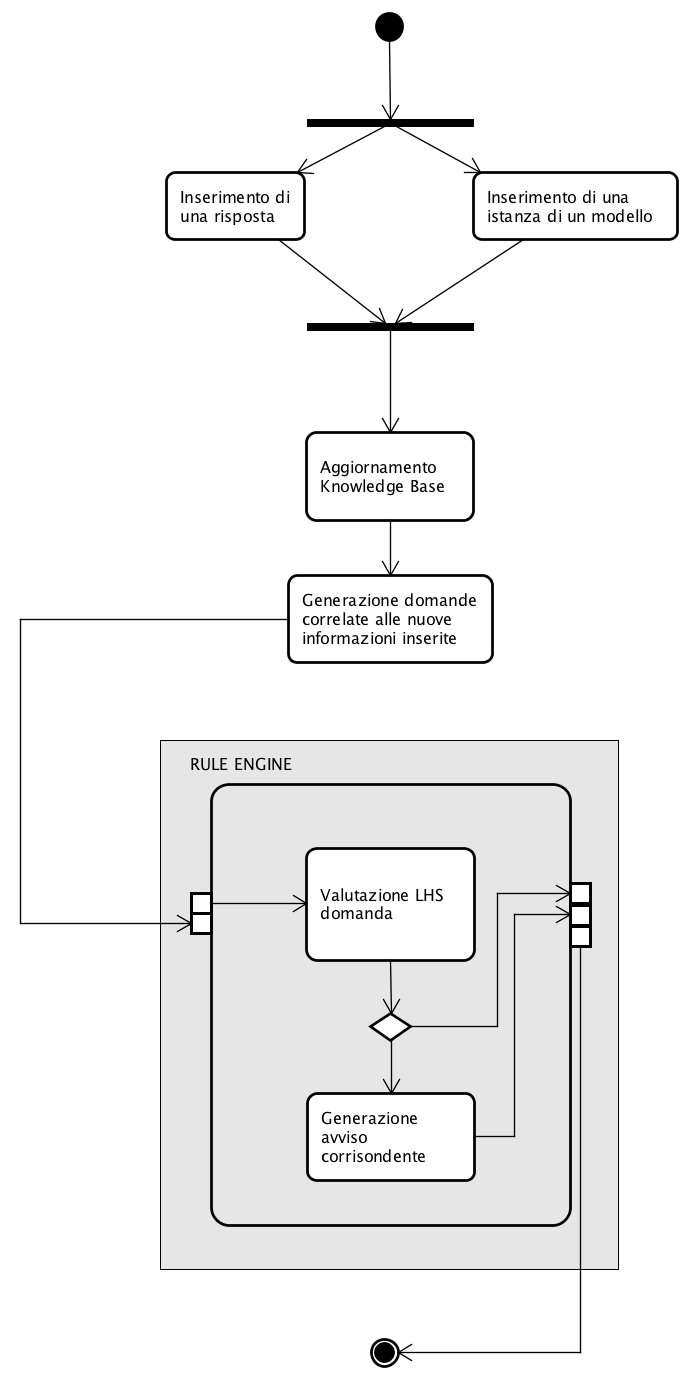
\includegraphics[width=10cm]{Pics/diagramma_attivita_risposte.png}
		\caption{Diagramma di attività del flusso di una risposta o l'inserimento di un oggetto a modello}
		\label{fig:DiagrammaAttivitaRisposte}
	\end{center}
\end{figure}





\section{Definizione dei casi d'uso}
	\subsection{Legenda}
	\subsection{UC 1}
	\subsection{UC 1.1}
	\subsection{UC 1.2}
	\subsection{UC 1.2.1}
	\subsection{UC 2}	
	\subsection{UC ...}

\section{Sviluppo}
\subsection{Refactor delle componenti esistenti}
	
\subsubsection{Refactor della componente: \textit{Figure di sistema}}
\subsubsection{Refactor della componente: \textit{Dispositivi di protezione individuale}}
\subsubsection{Refactor della componente: \textit{Mansioni e formazioni correlate}}
\subsection{Refactor della componente: \textit{Questionari}}


\subsection{Nuove componenti}
\subsubsection{\textit{Segnalazioni}}
	\paragraph{Requisiti}
	\paragraph{Progettazione}
	\paragraph{Criticità incontrate}
\subsubsection{\textit{Procedure}}
	\paragraph{Requisiti}
	\paragraph{Progettazione}
	\paragraph{Criticità incontrate}
\subsubsection{\textit{Dispositivi di protezione collettivi}}
	\paragraph{Requisiti}
	\paragraph{Progettazione}
	\paragraph{Criticità incontrate}


\subsection{Regole Drools}
	
\section{Verifica e validazione}
\section{Considerazioni finali}